\documentclass{ccr16}

% PACKAGES ---------------------------------------------------------------
\usepackage{amsfonts}
\usepackage{amsmath}
\usepackage{graphicx}
\usepackage{subfigure}

% ADD YOUR OWN PACKAGES HERE ---------------------------------------------
\usepackage{lipsum}
\usepackage[procnames]{listings}
\usepackage{color}
\usepackage{algorithm}
\usepackage{algpseudocode}
\usepackage[left = 1.5in, right = 1.5in]{geometry}

\definecolor{PDBM_keywords}{RGB}{255, 0, 90}
\definecolor{PDBM_comments}{RGB}{0, 0, 113}
\definecolor{PDBM_blue}{RGB}{0, 0, 160}
\definecolor{PDBM_red}{RGB}{160, 0, 0}
\definecolor{PDBM_green}{RGB}{0, 150, 0}
\definecolor{PDBM_orange}{RGB}{255, 165, 0}
    
\lstdefinestyle{PDBM_customc}
{
    language = C,
    belowcaptionskip = 0.3em,
    breaklines = true,
    frame = single,
    xleftmargin = \parindent,
    showstringspaces = false,
    basicstyle = \scriptsize\ttfamily,
    keywordstyle = \bfseries\color{PDBM_green},
    commentstyle = \itshape\color{PDBM_red},
    identifierstyle = \color{PDBM_blue},
    stringstyle = \color{PDBM_red},
    procnamekeys = {def, class},
    tabsize = 4
}

% DEFINITIONS ------------------------------------------------------------
% ADD YOUR OWN DEFINITIONS HERE ------------------------------------------
% BE SURE TO PREFACE LABEL WITH YOUR OWN INITIALS (SSS in this example) --
\newcommand{\PDBMnorm}[1]{\left\Vert#1\right\Vert}
\newcommand{\PDBMabs}[1]{\left\vert#1\right\vert}

% This controls the table-of-contents entry in the proceedings. Edit it
% to include your article title followed by the authors' names, as shown.
\addcontentsline{toc}{chapter}
{
    Accelerating DGM with Graphics Processing Units and Kokkos \\
    {\em P.D.\ Bello-Maldonado, C.\ Ober and K.\ Belcourt}
}

\pagestyle{myheadings}

\thispagestyle{plain}

% This gives the running head. Usually you list a shortened version of
% your article title (unless it's already very short) along with
% the author's names, as shown.
\markboth{GPU Acceleration of DGM}{P.D.\ Bello-Maldonado, C.\ Ober and K.\ Belcourt}

% Put your article title in here
\title{Accelerating DGM with Graphics Processing Units and Kokkos}

% List each author, their affiliation, and their e-mail address, as shown.
\author
{
    Pedro D.\ Bello-Maldonado\thanks{Dept. of Computer Science, University of Illinois at Urbana-Champaign, belloma2@illinois.edu} \and Curtis Ober\thanks{Sandia National Laboratories, ccober@sandia.gov} \and Kenneth Belcourt\thanks{Sandia National Laboratories, kbelco@sandia.gov}
}

\begin{document}

    \maketitle

    % Include your abstract here.
    \begin{abstract}
        Numerical computing has seen a rapid increase in the past several years as simulations became the go to approach for product development and scientific discovery. Implemented in DGM, the Discontinous Galerkin method is one of the most popular computing tools due to its versatility in adapting to meshes with mixed elements as well as better accuracy and general numerical properties. A GPU parallelization with Kokkos was added to DGM achieving improvements of twice the speed when considering the communication time and 20x the speed without communication. This initial implementation aims to serve as proof of concept in order to demonstrate how GPU computing can significantly improve the execution time of DGM for further development in the future.
    \end{abstract}

    \section{Introduction}
    {
        \label{PDBM:sec:intro}

        Given the rise of computing power over the last 50 years, computer simulations have become a key component in the development of new products and services. Companies save millions of dollars every year by testing their products using computers instead of building disposable prototypes. Furthermore, better and better simulation tools and methods are developed by scientists and engineers to improve the quality of the results and reduce the time to completion. This trend is seen in all sectors of the economy  from engineering to finance, and the demand for skilled workers in these fields is expected to grow significantly in the next years.

        While the computing resources are mostly available to anyone through funding agencies like NSF and the XSEDE program or private clusters, utilizing these resources can be daunting for non-computing experts. Furthermore, with newer computing architectures emerging every year it is hard to determine what the best option is when choosing a platform for running a particular simulation. Different systems offer different features that may be well suited for a specific application while being the wrong choice for a different one. Even if it is clear that a certain platform is the right choice for an application developing code to maximize resource usage is not possible without significant effort. For this reason, new programming tools that aim to overcome this issue are being developed to maximize the performance of applications while keeping it simple for non-experts to use. Compilers are also getting smarter and smarter at determining how code translates to machine instructions that make use of the resources effectively. In this work we focus on one of these tools named Kokkos used for GPU computing and a computing method known as the Discontinous Galerkin (DG) method for the solution of partial differential equations. Our main objective is to accelerate the execution time of a DG code using GPUs.

        The rest of this paper is organized as follows. In Section \ref{PDBM:sec:background} we introduce the DG method at a very high level and the code that implements it named DGM. Also a survey of GPU computing tools is listed as to understand where Kokkos lies in the spectrum of programming tools for GPUs. We present here the basics of the Kokkos library and show a simple example so the reader appreciates how easy it is to use. Section \ref{PDBM:sec:methodology} describes the approach used to accelerate a portion of DGM that fits well in the GPU programming paradigm. Results of our efforts are summarized in Section \ref{PDBM:sec:results} with plots of the speedups achieved, and finally we conclude our work in Section \ref{PDBM:sec:conclusions}.
    }

    \section{Background}
    {
        \label{PDBM:sec:background}

        In the realm of Scientific Computing, the numerical solution of partial differential equations (PDEs) is at the core of scientific discovery and product development. These equations describe many physical systems involving multiple independent and dependent variables, making them almost impossible to solve in closed form (i.e. the solution is given by a function or set of functions satisfying the equations exactly). Many numerical methods have been proposed to address this issue. The general approach in these methods is to decompose the domain (i.e. the physical space where the physics is happening) into many well defined, disjoint elements and use them to solve the equations at a set of discrete points (e.g. nodal methods). Other approaches aim to approximate the solution using interpolation where the unknowns become the coefficients in the interpolating function (e.g. modal methods) \cite{PDBM:Ciarlet02, PDBM:Constantine14, PDBM:Hutton03}.

        In either case the computational complexity of the method can be very expensive if the solution is to be very accurate. This can be done by increasing the number of elements, known as $h$-refinement, or increasing the polynomial degree of the basis functions in each element, known as $p$-refinement. Furthermore, for time evolving PDEs, different time-stepping approaches are possible that can be of explicit nature or implicit nature, each with its own advantages and disadvantages \cite{PDBM:Subbaraj89, PDBM:Dokainish89}.

        \subsection{The Discontinous Galerkin Method and DGM}
        {
            One of the numerical methods for the solution of PDEs is the Discontinous Galerkin Method or DG for short. DG methods combine features of the Finite Element method (FE) and the Finite Volume method (FV) to overcome the challenges each one has with respect to accuracy, $hp$-adaptivity, and explicit/implicit time-stepping. Solutions to the PDE are locally approximated in the Galerkin sense (i.e. the residual is minimized using the weighted residual formulation at each element) which causes discontinuous solutions at the interface of elements. In order to pick one solution fluxes are used as in the FV method and in this way the discretization is complete and the solution unique \cite{PDBM:Hesthaven08}.

            Many codes are available for the discretization of PDEs with DG. In this work we focus on DGM developed by Scott Collis and his students at Rice University and now maintained at Sandia National Laboratories. The code features discretization in space using mixed nodal and modal representations, as well as a suite of time integrators with many examples of different classes of PDEs (e.g. Navier-Stokes, advection-diffusion, Poisson, etc.) \cite{PDBM:Collis}.
        }

        \subsection{Parallel Computing and Accelerators}
        {
            Once the problem being solved gets too large to fit on a single machine or too expensive to run in a timely manner, high performance computing becomes the go to tool. In this computing paradigm, the problem is broken down and distributed across multiple processors that compute the solution in parallel. Significant speed improvements can be possible with enough computing units. Furthermore, specialized hardware designed to maximize computational throughput can be used to further accelerate the execution time of the application. Currently, two architectures are the most widely adopted in supercomputing clusters: graphics processing units (GPUs) and Intel Xeon Phi coprocessors (the newest version is not a coprocessor anymore. See Intel Knights Landing).

            Different programming tools are available for GPU computing. For NVIDIA GPUs the Compute Unified Device Architecture (CUDA) programming model is the standard for programming the accelerators \cite{PDBM:Nickolls08}. CUDA is an extension to the C/C++ language that supports GPU computing and provides routines to manage memory and run functions (called kernels) on the GPU. A similar tool that supports other GPU vendors, as well as NVIDIA, is the OpenCL library. Both of these tools work very close to the hardware and require the user to carefully map computational work to the manycore architecture on the GPU. Higher level programming libraries such as OpenACC and OpenMP make it easier and faster for programmers to write GPU code without worrying about the underlying architecture at the expense of performance \cite{PDBM:Wienke12, PDBM:OpenMP15}. In these cases the programmer instruments the sequential code with compiler directives that aid the compiler in deciding how to port the code to the GPU and run it.

            A third category of programming models for GPUs and other multithreaded architectures aims to use abstractions to describe the parallel computation so it can be run on different architectures. These tools provide a ``write once, run everywhere" approach  that enables parallelism without writing code for each different platform. Some examples include the Kokkos library in Trilinos \cite{PDBM:Heroux05}, VTK-m \cite{PDBM:Moreland16}, and Loo.py \cite{PDBM:Kloeckner14}. 
        }

        \subsection{The Kokkos Library}
        {
            Developed by Carter Edwards and Christian Trott at Sandia National Lab, the Kokkos library implements a programming model in C++ for writing performance portable applications targeting all major high performance computing (HPC) platforms \cite{PDBM:Edwards13}. Architectural features are abstracted so the user need not worry about the specifics of the platform the code is to be run on.

            Abstractions in Kokkos have the following forms:

            \begin{itemize}
                \item \textit{Memory Space}: Describes where the data resides (e.g. device memory, host memory)

                \item \textit{Execution Space:} Describes where the functions are executed (e.g. GPU, XeonPhi, CPU)

                \item \textit{Execution Policy:} Describes how and where a user function is executed (e.g. concurrently call function $f \left ( i \right )$ for $i = \left [ 0, n \right )$)

                \item \textit{Pattern:} Describes the execution pattern (e.g. parallel for, reduce, scan, or task)
            \end{itemize}

            In Listing \ref{PDBM:lst:kokkos_example} a simple example of Kokkos code is presented. The \texttt{Kokkos::View} object is a smart pointer that allocates memory on the memory space defined at compile time or specified in one of the template parameters. Then after that we launch a kernel on the GPU using \texttt{Kokkos::parallel\_for} with \texttt{num\_elem} threads and use the indexing to assign an initial value to each element in the array. In this way, we are letting Kokkos define the underlying distribution of thread blocks (or teams depending on the architecture) on the device. More specific distributions of threads can be possible for finer control, as well. On the other hand, notice that it is possible to change the memory space and execution space by just recompiling the code with the appropriate flags without changing the source code at all. For further details please refer to the Kokkos documentation.

            \lstinputlisting[caption = {Kokkos example}, label = {PDBM:lst:kokkos_example}, style = PDBM_customc]{./plots/PDBM_kokkos_example.cpp}
        }
    }

    \section{Methodology}
    {
        \label{PDBM:sec:methodology}

        In order to support a large number of elements during simulation, DGM was implemented in parallel with MPI. The code has been run on hundreds of thousands of processors effectively and has been tested in different platforms. However, little effort has been put into migrating portions of the code to GPUs. Under the right circumstances, significant improvements can be achieved with GPUs and in this section we explain our approach to parallelize DGM with GPUs and Kokkos.

        \subsection{Element Blocks}
        {
            Meshing a domain significantly impacts the performance of any numerical method for PDEs. Good meshes represent the physical domain as closely as possible, but using some element types may be too expensive or too hard to mesh. DGM supports mixed elements enabling a large number of possibilities for the programmer to achieve good representation. This feature in DGM allows for meshing portions of the domain with the exact same element while other portions may have more unstructured ones. Computationally speaking this is very efficient since many properties of the element are shared among identical elements thus reducing recomputing of such properties. An example of this is the Jacobian of the element which is used to map the local element to the reference element. In DGM, an \texttt{ElementBlock} class is provided for this purpose. All the elements in an \texttt{ElementBlock} object are aligned in memory as to facilitate accessing the data of all the elements with a single pointer. This is a key feature in the parallelization with GPUs since a single copy is possible from the host to the device without worrying about padding the field data of each element in a contigous array on the device.
        }

        \subsection{Functions of Interest}
        {
            Maximizing efficiency on GPUs in order to achieve excellent speedups is not always possible if the task being parallelized doesn't fit the computing paradigm. A good understanding of the code and the problem it solves is necessary before parallelization efforts are put in place. Here, we show the functions of interest that we propose to port to the GPU and their mathematical meaning.

            \subsubsection{The \texttt{inner\_product} Function}
            {
                For integration reasons, field data of each element needs to be multiplied by the basis functions in the discretization process. This is accomplished by the \texttt{inner\_product} function in DGM. Mathematically speaking the following steps achieve this. Let $q_{a}$, $q_{b}$, and $q_{c}$ be the quadrature points in the $x$, $y$, and $z$ directions, respectively. Also based on these quadrature points, the polynomial degrees of the basis functions take the form $L_{a} = q_{a} - 1$, $L_{b} = q_{b} - 1$, and $L_{c} = q_{c} - 1$. Let $\boldsymbol{u}^{\left ( e \right )}$ be a vector of size $q_{a} q_{b} q_{c}$ with the field values for element $e$ at the quadrature points, and $e = 1, \dots, E$ with $E$ being the total number of elements in the block. Let $\hat{\boldsymbol{u}}^{\left ( e \right )}$ be the vector of size $L_{a} L_{b} L_{c}$ with field values at the modes for each element. Finally, let $\mathrm{J}$ be the weighted Jacobian vector at the quadrature points and, $\boldsymbol{B}_{a}$ (size $L_{a} \times q_{a}$), $\boldsymbol{B}_{b}$ (size $L_{b} \times q_{b}$), and $\boldsymbol{B}_{c}$ (size $L_{c} \times q_{c}$) be the matrices used to project onto the basis functions. Algorithm \ref{PDBM:alg:inner_product} implements this procedure.

                \renewcommand{\algorithmicrequire}{\textbf{Input:}}
                \renewcommand{\algorithmicensure}{\textbf{Output:}}

                \begin{algorithm}[t]
                    \caption{\texttt{inner\_product} function description}

                    \begin{algorithmic}[1]
                        \Require Number of quadrature points in each dimension, $q_{a}$, $q_{b}$, and $q_{c}$. Number of modes in each dimension, $L_{a}$, $L_{b}$, and $L_{c}$. Weighted Jacobian of the element, $\mathrm{J}$. Matrices to project onto the basis functions, $\boldsymbol{B}_{a}$, $\boldsymbol{B}_{b}$, and $\boldsymbol{B}_{c}$. Field, $\boldsymbol{u}$, for each element. Number of elements, $E$. All matrices and vectors are assumed to be layed out in memory in row major ordering for reshaping purposes.

                        \Ensure Projected field onto the basis modes, $\hat{\boldsymbol{u}}$, for all the elements
                        \Procedure{\texttt{inner\_product}}{}
                            \For{$e = 1$ to $E$}
                                \State $\boldsymbol{u}_{w} = \textup{diag} \left ( \mathrm{J} \right ) \boldsymbol{u}^{\left ( e \right )}$
                                \State $\boldsymbol{U}_{w} = $ reshape $\boldsymbol{u}_{w}$ from $q_{a} q_{b} q_{c}$ to $q_{a} \times q_{b} q_{c}$
                                \State $\boldsymbol{H}^{\prime} = \boldsymbol{B}_{a} \, \boldsymbol{U}_{w}$
                                \State $\boldsymbol{H}^{\prime \prime} = $ zero matrix of size $L_{a} \times L_{b} q_{c}$
                                \For{$l_{a} = 1$ to $L_{a}$}
                                    \State $\boldsymbol{H}^{\left ( l_{a} \right )} = $ reshape $\boldsymbol{H}^{\prime \left ( l_{a} \right )}$ from $q_{b} q_{c}$ to $q_{b} \times q_{c}$
                                    \State $\boldsymbol{R} = \boldsymbol{B}_{b} \boldsymbol{H}^{\left ( l_{a} \right )}$
                                    \State $\boldsymbol{H}^{\prime \prime \left ( l_{a} \right )} = $ reshape $\boldsymbol{R}$ from $L_{b} \times q_{c}$ to $L_{b} q_{c}$
                                \EndFor

                                \State $\boldsymbol{H}^{\prime \prime} = $ reshape $\boldsymbol{H}^{\prime \prime}$ from $L_{a} \times L_{b} q_{c}$ to $L_{a} L_{b} \times q_{c}$
                                \State $\hat{\boldsymbol{U}} = \boldsymbol{H}^{\prime \prime} \boldsymbol{B}_{c}^{\top}$
                                \State $\hat{\boldsymbol{u}}^{\left ( e \right )} = $ reshape $\hat{\boldsymbol{U}}$ from $L_{a} L_{b} \times L_{c}$ to $L_{a} L_{b} L_{c}$
                            \EndFor
                            \State \Return $\hat{\boldsymbol{u}}$
                        \EndProcedure
                    \end{algorithmic}
                    \label{PDBM:alg:inner_product}
                \end{algorithm}
            }

            \subsubsection{The \texttt{backward\_transform} Function:}
            {
                While projecting field data onto the basis modes is accomplished with the \texttt{inner\_product} function, the inverse operation is possible, as well. This is what the \texttt{backward\_transform} function does. Using the same notation as before, Algorithm \ref{PDBM:alg:backward_transform} shows the implementation in this case.

                \renewcommand{\algorithmicrequire}{\textbf{Input:}}
                \renewcommand{\algorithmicensure}{\textbf{Output:}}

                \begin{algorithm}[t]
                    \caption{\texttt{backward\_transform} function description}

                    \begin{algorithmic}[1]
                        \Require Number of quadrature points in each dimension, $q_{a}$, $q_{b}$, and $q_{c}$. Number of modes in each dimension, $L_{a}$, $L_{b}$, and $L_{c}$. Matrices to project onto the basis functions, $\boldsymbol{B}_{a}$, $\boldsymbol{B}_{b}$, and $\boldsymbol{B}_{c}$. Projected field, $\hat{\boldsymbol{u}}$, for each element. Number of elements, $E$. All matrices and vectors are assumed to be layed out in memory in row major ordering for reshaping purposes.

                        \Ensure Field value on the grid points, $\boldsymbol{u}$, for all the elements
                        \Procedure{\texttt{backward\_transform}}{}
                            \For{$e = 1$ to $E$}
                                \State $\hat{\boldsymbol{U}} = $ reshape $\hat{\boldsymbol{u}}^{\left ( e \right )}$ from $L_{a} L_{b} L_{c}$ to $L_{a} \times L_{b} L_{c}$
                                \State $\hat{\boldsymbol{H}}^{\prime} = \boldsymbol{B}_{a}^{\top} \, \hat{\boldsymbol{U}}$
                                \State $\hat{\boldsymbol{H}}^{\prime \prime} = $ zero matrix of size $q_{a} \times q_{b} L_{c}$
                                \For{$q = 1$ to $q_{a}$}
                                    \State $\hat{\boldsymbol{H}}^{\left ( q \right )} = $ reshape $\hat{\boldsymbol{H}}^{\prime \left ( q \right )}$ from $L_{b} L_{c}$ to $L_{b} \times L_{c}$
                                    \State $\hat{\boldsymbol{R}} = \boldsymbol{B}_{b}^{\top} \hat{\boldsymbol{H}}^{\left ( q \right )}$
                                    \State $\hat{\boldsymbol{H}}^{\prime \prime \left ( q \right )} = $ reshape $\hat{\boldsymbol{R}}$ from $q_{b} \times L_{c}$ to $q_{b} L_{c}$
                                \EndFor

                                \State $\hat{\boldsymbol{H}}^{\prime \prime} = $ reshape $\hat{\boldsymbol{H}}^{\prime \prime}$ from $q_{a} \times q_{b} L_{c}$ to $q_{a} q_{b} \times L_{c}$
                                \State $\boldsymbol{U} = \hat{\boldsymbol{H}}^{\prime \prime} \boldsymbol{B}_{c}$
                                \State $\boldsymbol{u}^{\left ( e \right )} = $ reshape $\boldsymbol{U}$ from $q_{a} q_{b} \times q_{c}$ to $q_{a} q_{b} q_{c}$
                            \EndFor
                            \State \Return $\hat{\boldsymbol{u}}$
                        \EndProcedure
                    \end{algorithmic}
                    \label{PDBM:alg:backward_transform}
                \end{algorithm}
            }
        }

        \subsection{Parallelization}
        {
            As described, both Algorithm \ref{PDBM:alg:inner_product} and \ref{PDBM:alg:backward_transform}, can be parallelized in several ways. For starters, element computations are independent of each other. Each individual element could potentially be assigned to a thread and computed in parallel. Furthermore, the individual computations of each element are basic linear algebra routines that benefit from manycore architectures. Listing \ref{PDBM:lst:element_mul} and \ref{PDBM:lst:matrix_mul} show the implementation of two key portions of Algorithm \ref{PDBM:alg:inner_product}: multiplying the Jacobian by the field (an element to element vector multiplication that is represented as a diagonal matrix multiplied by a vector) and a simple matrix-matrix multiplication. A very similar code is used for \texttt{backward\_transform} since the math is effectively the same.

            \lstinputlisting[caption = {Element-to-element multiplication of the field, $\boldsymbol{u}$, by the weighted Jacobian, $\mathrm{J}$}, label = {PDBM:lst:element_mul}, style = PDBM_customc, float = tp]{./plots/PDBM_element_mul.cpp}

            In Listing \ref{PDBM:lst:element_mul} we see a couple of new Kokkos features not shown before. Mainly the \texttt{TeamPolicy} object. This object defines how threads are distributed and organized in teams. The number of teams and the number of threads per team is given in the constructor of the object. For each team, a \texttt{TeamThreadRange} object organizes the threads and gives them IDs to be referenced in the body of the function where they are used. The CUDA equivalent of teams and thread range, in this case, is thread blocks and threads in a one dimensional configuration. Kokkos manages the mapping automatically and takes care of the correct indexing at the boundaries. Finally, in the body of the function each element is indexed by \texttt{e * (q\_a * q\_b * q\_c)} and each quadrature point is multiplied by the Jacobian. Notice that this is only possible because the elements in an \texttt{ElementBlock} have consecutive memory addresses separated by blocks of size $q_{a} q_{b} q_{c}$. We are not showing the view allocation here, but it suffices to say that \texttt{u} and \texttt{wJ} reside in global memory on the device and have the correct data.

            \lstinputlisting[caption = {Matrix-matrix multiplication of the basis function matrix and the reshaped Jacobian-multiplied field}, label = {PDBM:lst:matrix_mul}, style = PDBM_customc, float = tp]{./plots/PDBM_matrix_mul.cpp}

            For Listing \ref{PDBM:lst:matrix_mul}, a basic matrix-matrix multiplication is implemented for each element. The structure is similar to that of the element-to-element multiplication code but another layer of parallelism is included. The \texttt{ThreadVectorRange} object adds an extra dimension to the thread teams. For that reason in the constructor of the \texttt{TeamPolicy} object two arguments are given defining the block size in each dimension. The Kokkos library computes the number of blocks necessary to cover the ranges in \texttt{TeamThreadRange} and \texttt{ThreadVectorRange}, automatically. In the body of the function, a simple loop is used to compute each element of the output matrix which is the equal to the inner product of a row of the first matrix dotted with the column of the second matrix. In this way, the order of operations does not affect the value of the output compared to the sequential implementation and both values should be exactly the same. This was not by design and some accuracy could be sacrificed in spite of more parallelism but that is left for future optimizations of the code. The remaining portions of the routine have similar implementations and thus are not shown here.
        }
    }

    \section{Results}
    {
        \label{PDBM:sec:results}

        Our tests were run on the Shannon test bed in interative mode. The specifications per node are:

        \begin{itemize}
            \item Two 8-core Sandy Bridge Xeon E5-2670 @ 2.6GHz
            \item 128GB DDR3-1600MHz
            \item 2x NVIDIA K20 GPUs

            \begin{itemize}
                \item 2688 CUDA Cores
                \item 732MHz Clock rate
                \item 5760MB Global memory
            \end{itemize}

            \item RHEL 6
        \end{itemize}

        We performed 5 runs of each test and averaged the results. In analyzing the effectiveness of our algorithm, the number of elements is varied as well as the polynomial degree of the basis functions in each element. DGM provides an executable to generate a cubic mesh with hex elements of the same structure. Listing \ref{PDBM:lst:mesh_gen} shows the command to generate a computational mesh. Notice that the code generates a linear grid of elements of size $1 \times 1 \times 1$ in the $x$-direction. Other testings with a cubic grid of elements did not influence the speedups and the results were equivalent.

        \lstinputlisting[caption = {Mesh generation with DGM (Python string formating)}, label = {PDBM:lst:mesh_gen}, style = PDBM_customc]{./plots/PDBM_mesh_gen.py}

        \begin{figure}[h]
            \centering
            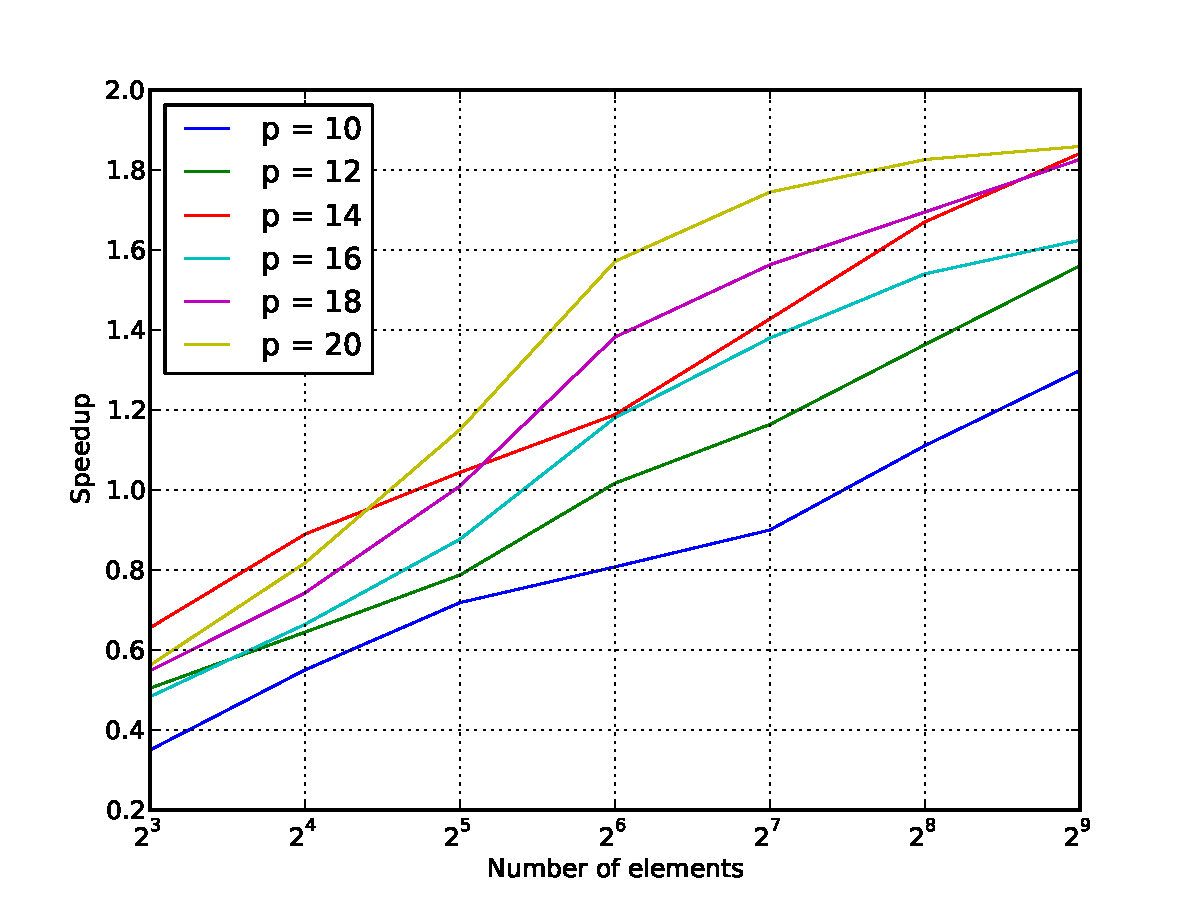
\includegraphics[trim = {0in 0.3in 0in 0.3in}, width = 0.5 \textwidth]{./plots/PDBM_speedup_inner.pdf}
            \caption{Overall speedup of \textup{inner\_product} function}
            \label{PDBM:fig:speedup_inner}
        \end{figure}
        ~
        \begin{figure}[h]
            \centering
            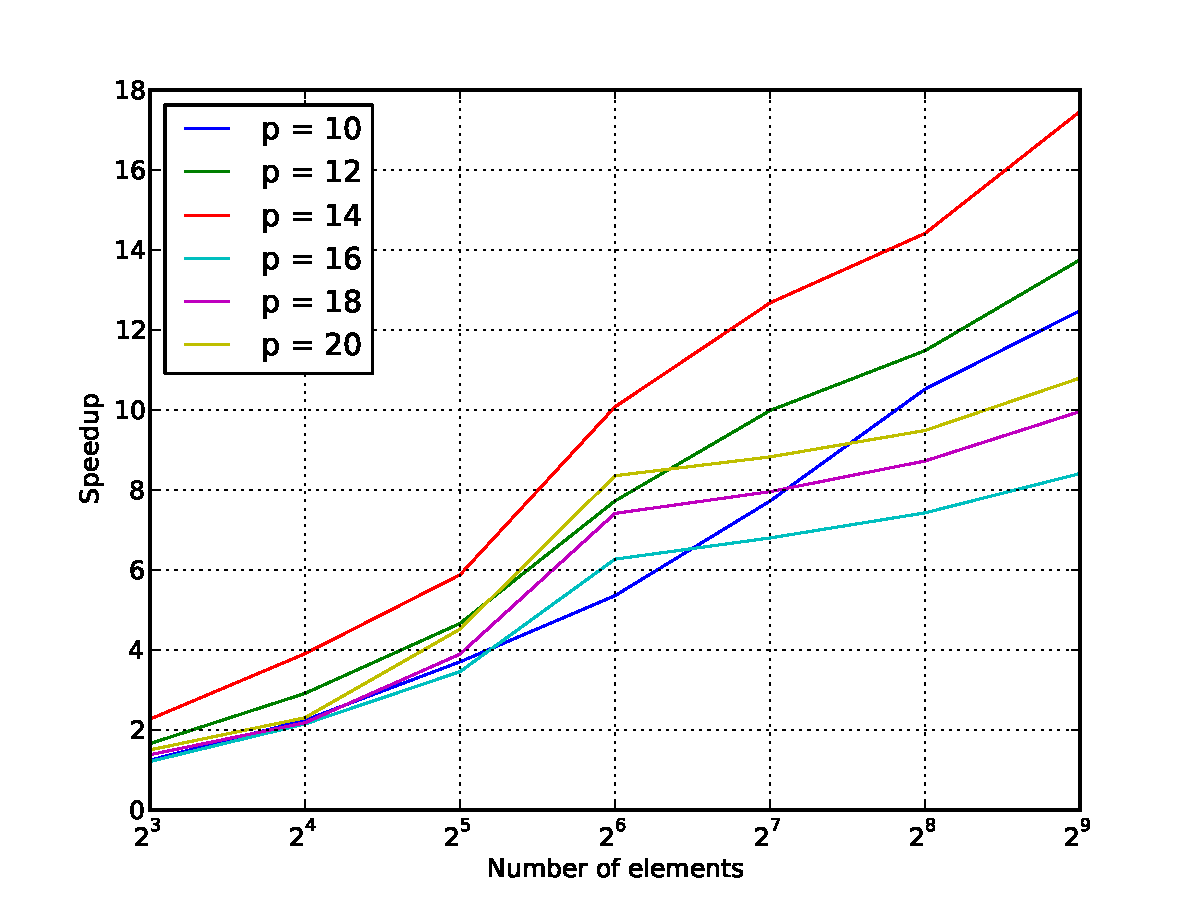
\includegraphics[trim = {0in 0.3in 0in 0.3in}, width = 0.5 \textwidth]{./plots/PDBM_speedup_no_comm_inner.pdf}
            \caption{Speedup of \textup{inner\_product} function without communication}
            \label{PDBM:fig:speedup_no_comm_inner}
        \end{figure}

        \begin{figure}[h]
            \centering
            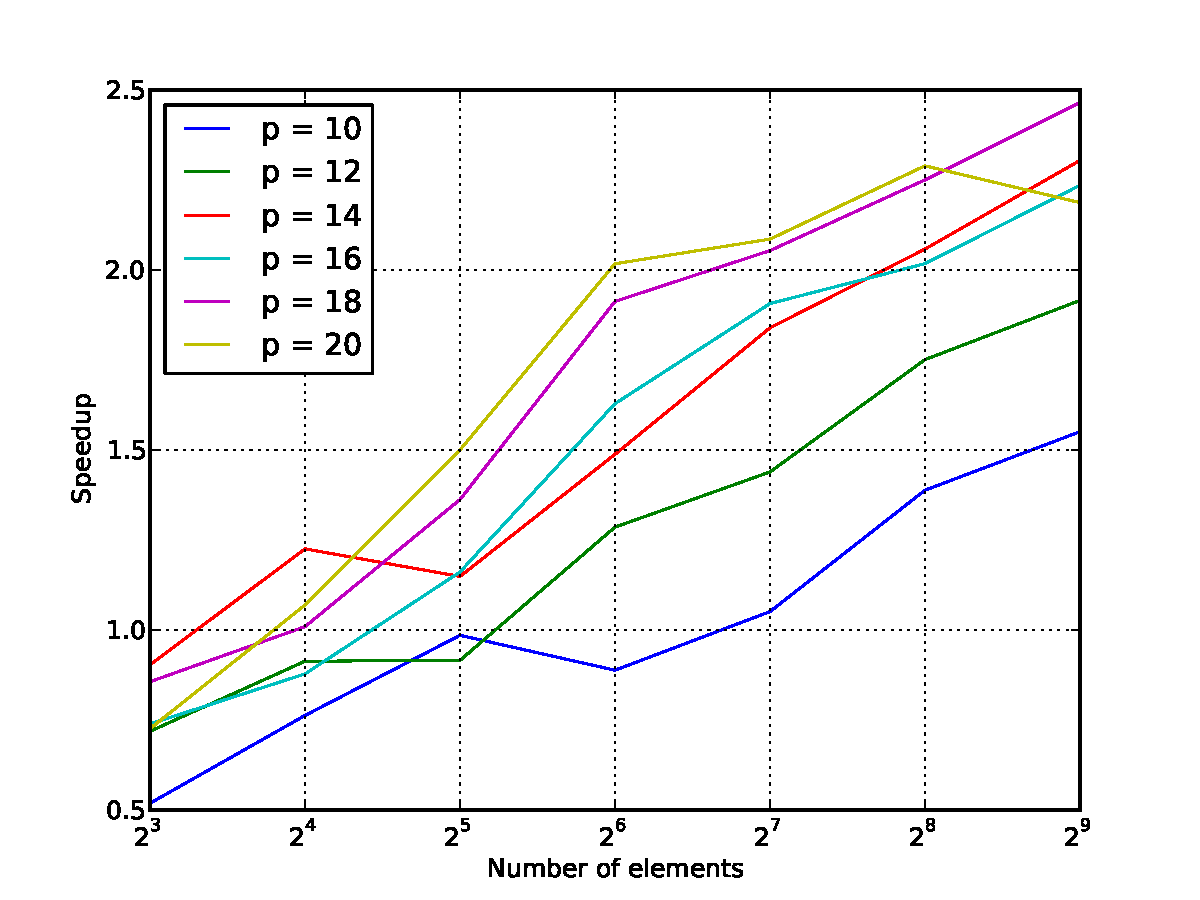
\includegraphics[trim = {0in 0.3in 0in 0.3in}, width = 0.5 \textwidth]{./plots/PDBM_speedup_backward.pdf}
            \caption{Overall speedup of \textup{backward\_transform} function}
            \label{PDBM:fig:speedup_backward}
        \end{figure}

        \begin{figure}[h]
            \centering
            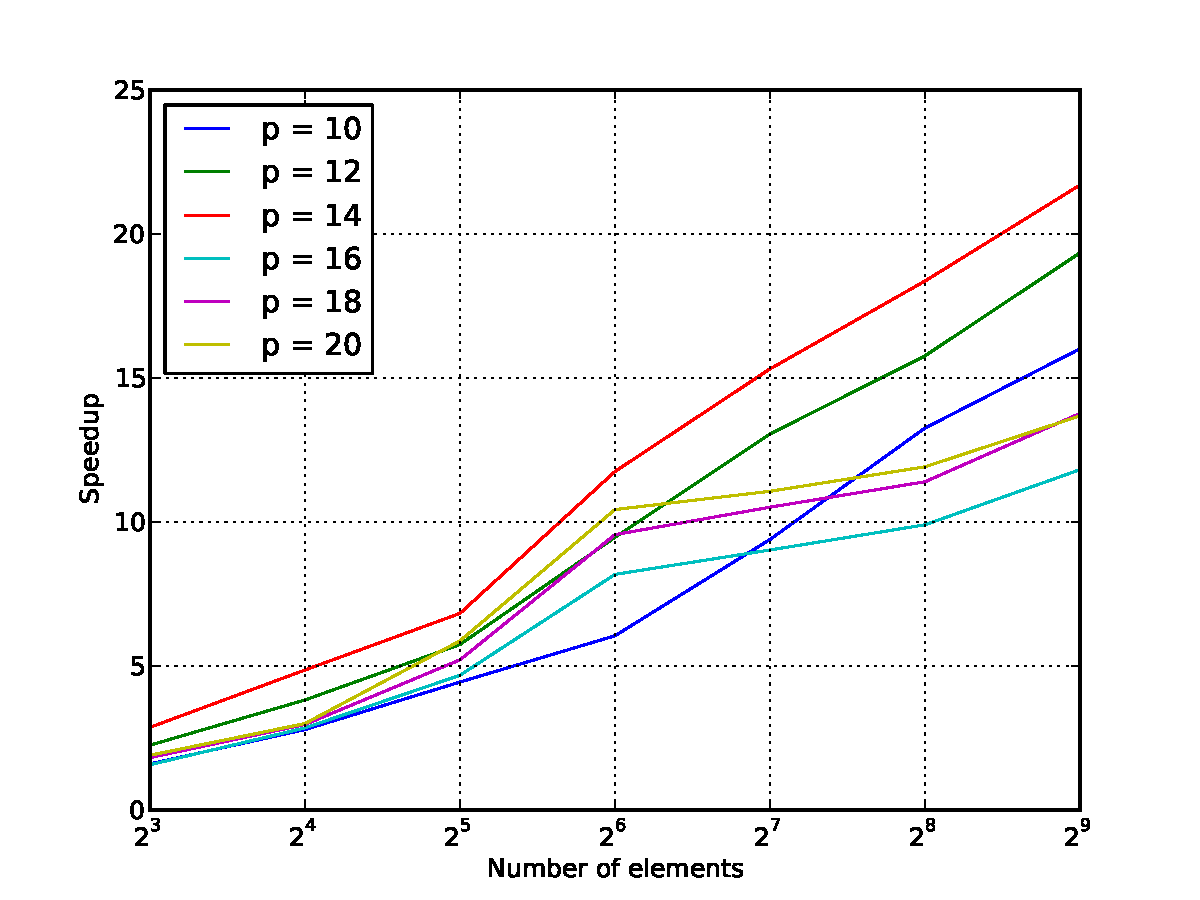
\includegraphics[trim = {0in 0.3in 0in 0.3in}, width = 0.5 \textwidth]{./plots/PDBM_speedup_no_comm_backward.pdf}
            \caption{Speedup of \textup{backward\_transform} function without communication}
            \label{PDBM:fig:speedup_no_comm_backward}
        \end{figure}

        Figures \ref{PDBM:fig:speedup_inner}-\ref{PDBM:fig:speedup_no_comm_backward} show the measured speed improvements for a \texttt{HexBlock} of size 8, 16, 32, 64, 128, 256, and 512, with and without the cost of communication for both functions of interest. In this case, communication means the data transfer between the CPU and the GPU. As we can see, with more grid points to work with, the speed improvement increases since the communication cost has less effect on the overall computation. Furthermore, a higher polynomial degree also means better performance, as a higher polynomial means more grid points per element. However, this trend is not seen when the communication cost is not taken into account. As we can see from Figure \ref{PDBM:fig:speedup_no_comm_inner} or \ref{PDBM:fig:speedup_no_comm_backward} the configuration with the best performance is a hex element with $p = 14$. This is true regardlessof the number of elements. We believe that, due to the fact that $p = 14$ means $p + 2 = 16$ grid points in each direction, an element with $16^{3} = 4096$ grid points fits exactly in one memory page and so it is very efficient, but further investigation is needed.

        When looking at the overall execution and not just each individual function an overall speedup gain is also achieved under the right conditions. Figure \ref{PDBM:fig:overall_performance} shows these results. As we can see, a total of 5\% improvement is seen for a run with 1000 time-steps. We expect that with more portions of the code ported to the GPU larger improvements will be seen.

        \begin{figure}[h]
            \centering
            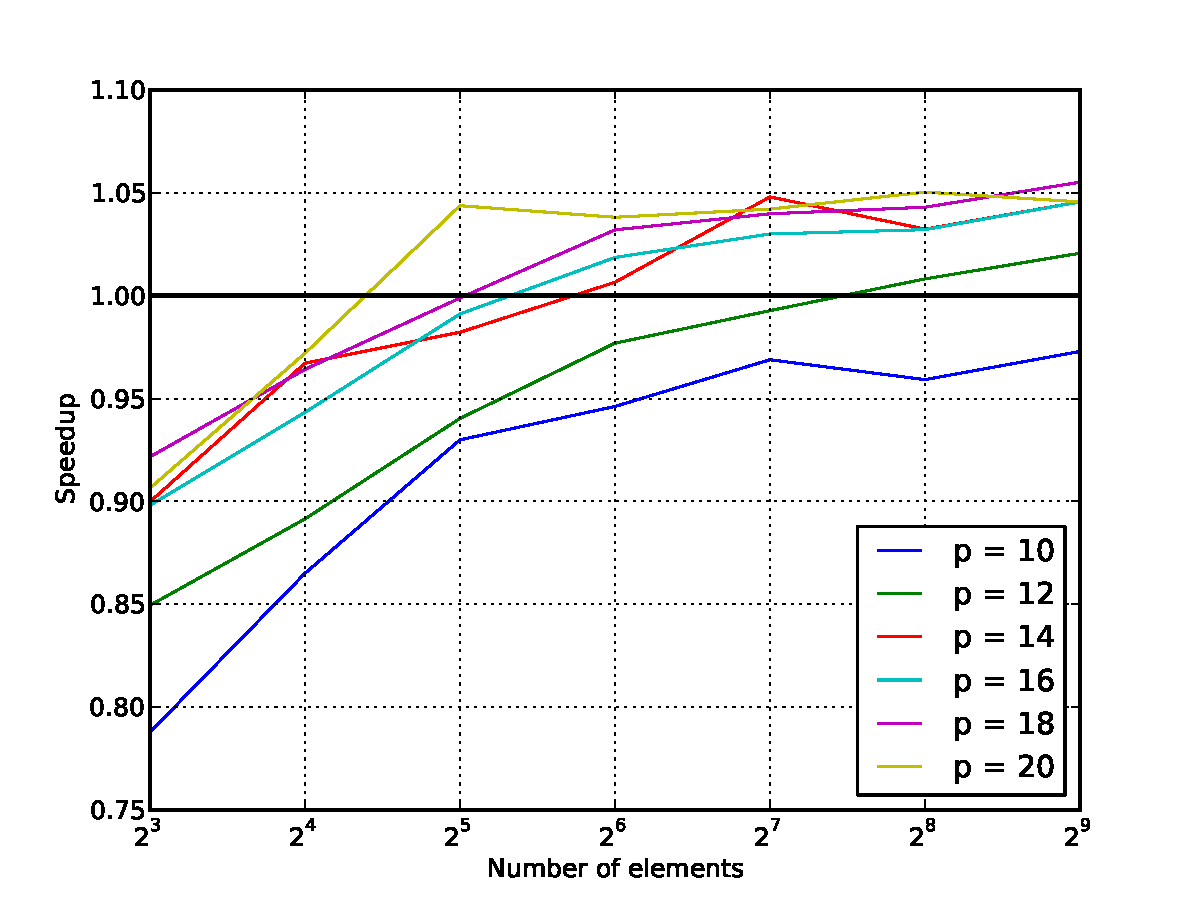
\includegraphics[trim = {0in 0.3in 0in 0.3in}, width = 0.5 \textwidth]{./plots/PDBM_overall_performance.pdf}
            \caption{Total performance gain for a test run with 1000 time-steps. Time measured from the beginning of the application to the end including all aspects of the execution (e.g. reading input files, setup, etc)}
            \label{PDBM:fig:overall_performance}
        \end{figure}
    }

    \section{Conclusions}
    {
        \label{PDBM:sec:conclusions}

        Numerical applications benefit greatly from the computing power of GPUs since computation can be broken into small, lightweight pieces that can be mapped efficiently onto the many core architecture of the GPU. However, in order to maximize performance, a careful mapping of the tasks is needed and this can't be done without significant understanding of the architecture. Tools like Kokkos facilitate the parallelization process by abstracting the hardware and generalizing parallel work so multiple platforms can be covered. We showed that improvements of twice the speed are possible even when the communication is present and a relatively low number of elements are available. The results show that increasing the total amount of work manifests into higher speedups. Furthermore, if communication is ignored huge improvements are seen since transferring data from the CPU to the GPU is the bottleneck of GPU computing in general. Future generations of GPUs will share the memory space with the CPU so we expect to see even faster GPU code in the near future. On the other hand, this initial approach to GPU parallelization of DGM aims to demonstrate how GPUs can be used with Kokkos in accelerating the application. Based on the results obtained, we can move forward and target more portions of the code that fit well on the GPU and expect to see a reduced computing time of DGM as a whole.
    }

    \bibliographystyle{siam}
    % Edit the line below to be your first and last names.
    \bibliography{kokkos}

    % Edit PedroBello-Maldonado below to be your first and last names, but leave the line commented out.
    % This line will help me merge bibliographies for the proceedings.
    %\input{PedroBello-Maldonado.bbl}

\end{document}
